%coding : UTF-8

% Hellotex.tex
%first edit 2023 4.9
%second edit 2023 6.29
\documentclass [UTF8] {ctexart}
\usepackage{geometry}%文件格式包‘
\geometry{a4paper,left=25mm,right=20mm,top=25mm,bottom=25mm}

\usepackage{fancyhdr}%页眉设置包
\pagestyle{fancy}
\fancyhf{}
\fancyhead[L]{}
\fancyhead[R]{}
\renewcommand{\headrulewidth}{0.9pt}
\cfoot{\thepage}

\usepackage{ctex}


\usepackage{graphicx}
\usepackage{makecell}
\usepackage{float}

\usepackage{amsmath}%数学宏包
\usepackage{bm}%公式加粗




\usepackage{pdfpages}%实现导入pdf


\CTEXsetup[format={\Large\bfseries}]{section}                        %设置章标题字号为Large,居左
\CTEXsetup[number={\chinese{section}}]{section}                      %section形式改为一,二,三,.. 
\CTEXsetup[name={(,)}]{subsection}                                 
\CTEXsetup[number={\chinese{subsection}}]{subsection}                %subsection形式改为(一,二,三,...)                            
\CTEXsetup[number=\arabic{subsubsection}]{subsubsection}             %subsubsection形式改为1,2,3,...
\newcommand{\subsubsubsection}[1]{\paragraph{#1}\mbox{}\\}
\setcounter{secnumdepth}{4} % how many sectioning levels to assign numbers to
\setcounter{tocdepth}{4} % how many sectioning levels to show in ToC


\bibliographystyle{plain}

\begin{document}

\begin{titlepage}	
% 封面信息
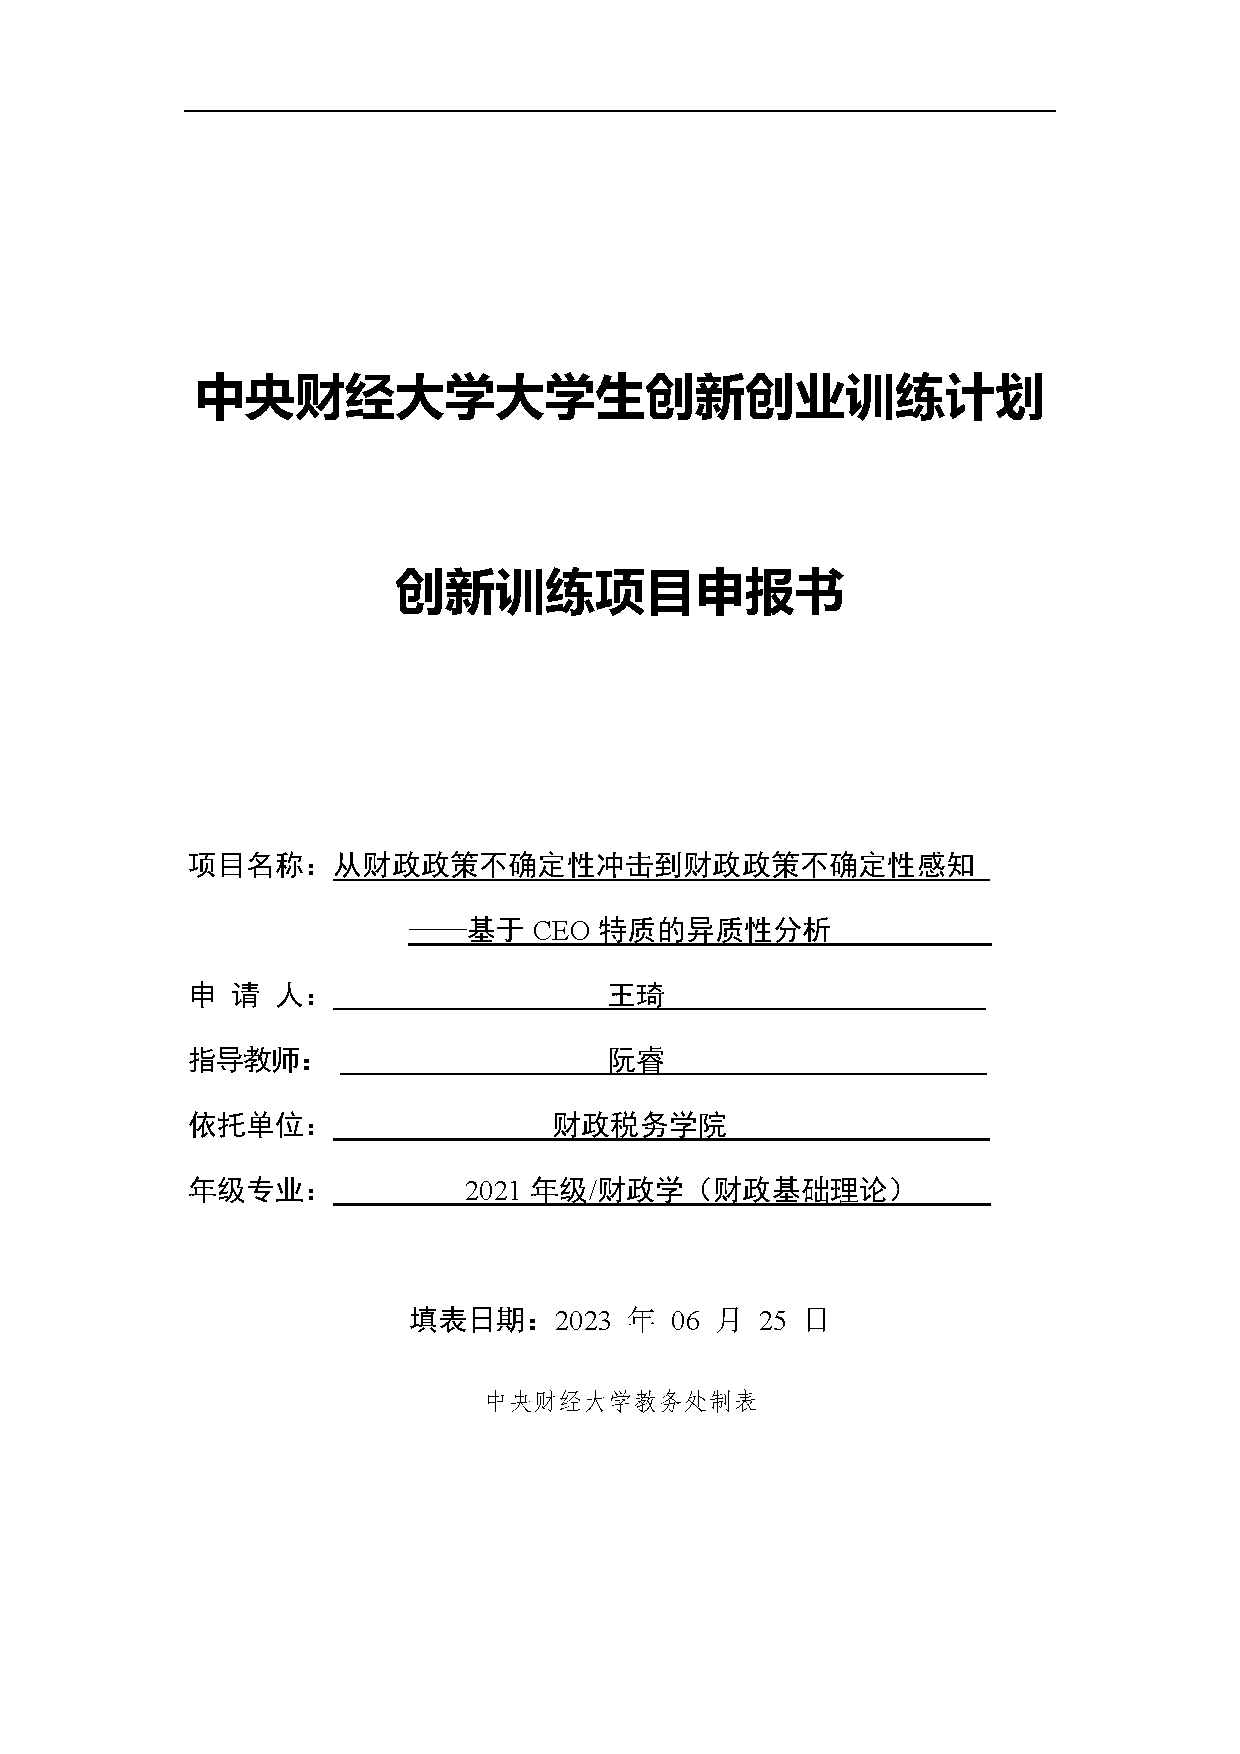
\includepdf[pages={1}]{cover.pdf} 
\includepdf[pages={2}]{cover.pdf} 
\includepdf[pages={3}]{cover.pdf} 
%曲线救国的思路,外界自建封面,然后调用

\tableofcontents
\thispagestyle{empty}%目录页不现实页码

\newpage
\setcounter{page}{1}%从正文开始计数
\end{titlepage})
\section{项目选题}
\subsection{选题背景}
\subsubsection{十四届全国人大政府工作报告强调推动“稳增长、稳就业、稳物价、稳预期”工作}

\subsubsection{精准财政政策靠前发力,惠企惠民}

\subsubsection{我国企业面临不确定性因素众多,企业发展受阻}

\subsubsection{探究企业对于财政政策不确定性的感知,符合我国发展需要}

\subsection{选题目的 }
\subsubsection{关注时事热点,契合“稳预期”发展}

\subsubsection{探究原因,深入剖析}

\leftline{(1)财政政策不确定性指数}

\leftline{(2)企业经济政策不确定性指数}


\subsubsection{立足现实,分析可行性}
\leftline{(1)理论可行性}



\leftline{(2)效果可行性}


\subsubsection{总结症结,提出建议}

\subsection{选题内涵和价值}
\subsubsection{微观视角切入,充实现有研究}


\subsubsection{契合“稳中求进”方针,唤醒企业活力}


\subsubsection{反映政策成效,为完善政策建言献策}


\subsubsection{定性定量分析,全面解读数据}


\section{研究或实践基础}
\subsection{从经济政策不确定性到企业财政政策不确定性}


FFPU 的计算如下,其中$I_P$ (s) 是示性函数,当$s\in P$时,I=1; 当$s\notin P$时,I=0 :
\bm{$${FFPU}_{it} = {\sum_{s~ = ~1}^{S_{it}}{n_{s}I_{P}(s)/N}}$$}


\subsubsection*{参考文献}
\addcontentsline{toc}{subsection}{参考文献}%添加不编号章节
代昀昊、孔东民(2017):《高管海外经历是否能提升企业投资效率》,《世界经济》第1期。

何瑛、于文蕾、戴逸驰、王砚羽(2019):《高管职业经历与企业创新》,《管理世界》第11期。



Stein, L. C., \& Stone, E. (2013). “The effect of uncertainty on investment, hiring, and R\&D: Causal evidence from equity options”. Hiring, and R\&D: Causal Evidence from Equity Options (October 4, 2013).

Veronesi, U., Orecchia, R., Maisonneuve, P., Viale, G., Rotmensz, N., Sangalli, C., ... \& Ballardini, B. (2013). 

“Intraoperative radiotherapy versus external radiotherapy for early breast cancer (ELIOT): a randomised controlled equivalence trial”. The lancet oncology, 14(13), 1269-1277.
\section{研究内容设计}

\section{项目保障}
\subsection{项目人员简介}

    \begin{tabular}{|p{5em}|p{35em}|}
    \hline
        
       \makecell[c]{项目人员}  & \makecell[c]{个人优势、科研经历及成果} \\ \hline
        \makecell[c]{王琦}&  财政税务学院2021级本科生,现为中国财政发展协同创新中心财政基础理论基地班成员,学习成绩优异。对学术研究有强烈兴趣,专业知识扎实,已学微观计量经济学等课程,能够掌握运用stata、Python、R、Latex等软件。曾担任多位协同中心老师的助研工作,助研工作十余项,在阮睿老师的《购买美国法案》研究课题下负责整理收集数据、撰写报告,在王麒植老师的指导下主持《财政学》教材整理工作,在姚东旻教授的课题组下参与案例编写,有较强的科研经验和组织领导能力。同时积极参加互联网+等学术科研创新创业比赛提高学术研究能力。  \\ \hline
        \makecell[c]{吴司锴} & 财政税务学院 2022级本科生,对学术研究有强烈兴趣,现为中国财政发展协同创新中心基地班成员。专业知识扎实,已自学统计学、微观计量经济学等课程,熟练使用 SPSS、stata、Python 等软件。 大一绩点排名班级前列,积极参与“模拟市长”等学术科研创新创业比赛锻炼能力,曾担任多位协同中心老师的科研助研,参与“地方城投与融资租赁,市域财政预算整理,《万历会计录》转录,‘购买美国’法案研究”等课题之中,在研究中夯实基本功。”也参与了“用英语讲中国故事比赛”并荣获北京市一等奖。善于思考问题寻找答案,擅长团队合作沟通,积极融入团队,发挥自身优势取长补短。现担任学院文体部部长,有良好的组织能力。 \\ \hline
        \makecell[c]{陆知雨} & 财政税务学院2022级本科生,现担任班级学习委员,对财经类学术研究抱有浓厚兴趣;本人有扎实的学科知识,掌握stata,latex,spss等多种计算机技术;积极参加学术实践,曾在购买美国法案研究,市域财政预算整理,《万历会计录》转录等多项科研项目中担任助研工作;学习兴趣浓厚,积极参加:互联网+,模拟市长等多项创新创业类比赛,并锻炼自己的能力;较强的学习能力、上进心强,处事态度细心谨慎、认真负责;富有团队合作精神,善于与他人沟通交流,尤其是技术方面的知识,虚心请教他人,共同学习,共同进步;有良好的生活习惯,与他人相处融洽,善于与人交际。 \\ \hline
    \end{tabular}
 
    


\subsection{项目经费预算}

\centering
    \begin{tabular}{|c|c|c|c|c|c|p{2em}|}
    \hline
        序号 & 预算科目 & 单位价格 & 数量 & 合计 (元) & 备注 \\ \hline
        1 & 电子文献下载及购买费用 & 20 & 30 & 400  &\thead{主要为国内外学者\\研究文献及经典期\\刊文献}\\ \hline
        2 & 线上课程及讲座费用 & 100 & 5 & 500  & \thead{相关课程讲座} \\ \hline
        3 & 笔 & 3 & 40 & 100  &   \\ \hline
        4 & 笔记本 & 20 & 5 & 100  &   \\ \hline
        5 & 文件夹 & 15 & 10 & 100  &   \\ \hline
        6 & 资料及报告打印费用 & 0.1/张 & 2000 & 200  &   \\ \hline
        7 & 数据库账户购买费用 & 300 & 1 & 300  &   \\ \hline
        8 & 交通费用 & 100/人 & 3 & 300  & \thead{两校区之间往返;\\参加研讨会等交通\\费用} \\ \hline
        总 计 & \multicolumn{5}{c|}{2000} \\ \hline
    \end{tabular}


\end{document}












